\documentclass{report}
    \title{50004 - Operating Systems - Lecture 14}
    \author{Oliver Killane}
    \date{18/12/21}
%===========================COMMON FORMAT & COMMANDS===========================
% This file contains commands and format to be used by every module, and is 
% included in all files.
%===============================================================================

%====================================IMPORTS====================================
\usepackage[a4paper, total={6in, 8in}]{geometry}
\usepackage{graphicx, amssymb, amsfonts, amsmath, xcolor, listings, tcolorbox, multirow, hyperref}
%===============================================================================

%====================================IMAGES=====================================
\graphicspath{{image/}}

% \centerimage{options}{image}
\newcommand{\centerimage}[2]{\begin{center}
    \includegraphics[#1]{#2}
\end{center}}
%===============================================================================

%=================================CODE LISTINGS=================================
\definecolor{codebackdrop}{gray}{0.9}
\definecolor{commentgreen}{rgb}{0,0.6,0}
\lstset{
    inputpath=code, 
    commentstyle=\color{commentgreen},
    keywordstyle=\color{blue}, 
    backgroundcolor=\color{codebackdrop}, 
    basicstyle=\footnotesize,
    frame=single,
    numbers=left,
    stepnumber=1,
    showstringspaces=false,
    breaklines=true,
    postbreak=\mbox{\textcolor{red}{$\hookrightarrow$}\space}
}

% Create a code listing for a single line
% \codeline{language}{line}{file}
\newcommand{\codeline}[3]{\lstinputlisting[language=#1, firstline = #2, lastline = #2]{#3}}

% Create a code listing for a given language & file
% \codelist{language}{file}
\newcommand{\codelist}[2]{\lstinputlisting[language=#1]{#2}}
%===============================================================================

%================================TEXT STRUCTURES================================
% Marka a word as bold
% \keyword{important word}
\newcommand{\keyword}[1]{\textbf{#1}}

% Creates a section in italics
% \question{question in italics}
\newcommand{\question}[1]{\textit{#1} \\ }

% Creates a box with title for side notes.
% \sidenote{title}{contents}
\newcommand{\sidenote}[2]{\begin{tcolorbox}[title=#1]#2\end{tcolorbox}}

% Creates an item in an itemize or enumerate, with a paragraph after
% \begin{itemize}
%     \bullpara{title}{contents}
% \end{itemize}
\newcommand{\bullpara}[2]{\item \textbf{#1} \ #2}

% Creates a compact list (very small gaps between items)
% \compitem{
%     \item item 1
%     \item item 2
%     \item ...
% }
\newcommand{\compitem}[1]{\begin{itemize}\setlength\itemsep{-0.5em}#1\end{itemize}}

% Creates a link to the lecture for use at the start of the notes document
\newcommand{\lectlink}[1]{\sidenote{Lecture Recording}{
    Lecture recording is available \href{#1}{here}
}}
%===============================================================================


%==============================SYNTAX HIGHLIGHTING==============================
\newcommand{\fun}[1]{\textcolor{blue}{\textbf{#1}}}
\newcommand{\file}[1]{\textcolor{green}{\textbf{#1}}}
\newcommand{\struct}[1]{\textcolor{orange}{\textbf{#1}}}
\newcommand{\var}[1]{\textcolor{purple}{\textbf{#1}}}
\newcommand{\const}[1]{\textcolor{red}{\textbf{#1}}}
%===============================================================================

%==============================THREAD HIGHLIGHTING==============================
\newcommand{\threada}[1]{\textcolor{green}{\textbf{#1}}}
\newcommand{\threadb}[1]{\textcolor{red}{\textbf{#1}}}
%===============================================================================

%============================DISPLAYING THREAD CODE=============================
\newcommand{\threadlist}[3]{
    \codelist{#1}{#2 init.#3}
    \begin{minipage}[t]{0.45\textwidth}
        \codelist{#1}{#2 A.#3}
    \end{minipage}
    \hfill
    \begin{minipage}[t]{0.45\textwidth}
        \codelist{#1}{#2 B.#3}
    \end{minipage}
}
%===============================================================================
\begin{document}
    \maketitle
    \lectlink{https://imperial.cloud.panopto.eu/Panopto/Pages/Viewer.aspx?id=33858a27-ea6d-4e5c-a6e8-adf0010414ac}

    \section*{Disk Scheduling}
        \subsection*{(FCFS) First Come First Served}
            Requests completed in the order they were received.
            \compitem{
                \item For light loads this is fine (time between requests is much larger than time taken to fulfil any request).
                \item Low performance for heavy loads (ends up traversing the disk more than optimal to get each request).
                \item Fair (no bais towards any process).
            }
            For example:
            \\ Head at $50$. Queue: $195, 365, 75, 245, 30, 260, 125, 135$
            \\ Operations: $50 \to 195 \to 365 \to 75 \to 245 \to 30 \to 260 \to 125 \to 135$
            \centerimage{width=\textwidth}{fcfs.png}

        \subsection*{(SSTF) Shortest Seek Time First}
            Order requests according to shortest seek distance from the current head position
            \compitem{
                \item Baised against innermost and outermost tracks (middle tracks on average closer, even with random head positions)
                \item Unpredictable performance (Requests may face a long delay if several very close requests are serviced)
                \item Processes can use dummy requests to keep control of head and have their requests prioritised.
                \item Can delay requests indefinitely (e.g many requests come in very close to eachother, trapping the head).
            }
            Head at $50$. Queue: $195, 365, 75, 245, 30, 260, 125, 135$
            \\ Operations: $50 \to 30 \to 75 \to 125 \to 135 \to 195 \to 245 \to 260 \to 365$
            \centerimage{width=\textwidth}{sstf.png}
        
        \subsection*{SCAN Scheduling}
            Also called elevator scheduling. Select requests with the shortest seek time in the preferred direction.
            \compitem{
                \item Only change direction when at the outermost/innermost cylinder (no more requests in the direction)
                \item Long delays for requests that are not in the path of the algorithm (e.g come in just behind the head) and for the extremes.
                \item Base for the most common algorithms used.
                \item Suffers from same delay issue as \keyword{SSTF}, though reduced (only in one direction)
            }
            Head at $160$. Queue: $195, 365, 75, 245, 30, 260, 125, 135$
            \\ Operations: $160 \to 195 \to 240 \to 260 \to 365 \to 135 \to 125 \to 75 \to 30$
            \centerimage{width=\textwidth}{scan.png}

        \subsection*{C-SCAN Scheduling}
            Much like \keyword{SCAN} but scanning in one direction only, jumping to the start (e.g innermost) when at the end (e.g outermost)
            \compitem{
                \item Lower variance of requests on extreme tracks
                \item Largely reduces issue of indefinite wait from \keyword{SSTF}.
            }
            Head at $160$. Queue: $195, 365, 75, 245, 30, 260, 125, 135$
            \\ Operations: $160 \to 195 \to 240 \to 260 \to 365 \to 30 \to 75 \to 125 \to 135$
            \centerimage{width=\textwidth}{c-scan.png}
        
        \subsection*{N-Step SCAN Scheduling}
            Same as \keyword{SCAN}, however only services requests waiting when the sweep began (for each sweep)
            \compitem{
                \item Requests arriving during sweep are serviced before end of the sweep (no long waits)
                \item No indefinite waits possible.
            }
            Head at $160$. Queue: $195, 365, 75, 245, 30$ Then $260, 125, 135$
            \\ Operations: $160 \to 195 \to 245 \to 365 \to 75 \to 30 \to (new \ sweep) \ 125 \to 135 \to 260$
            \centerimage{width=\textwidth}{n-step scan.png}

    \section*{Linux Disk Scheduling}
        \sidenote{struct bio}{
            Can be found \href{https://github.com/torvalds/linux/blob/3f667b5d4053ad54aee13dab5c94f04ff75ddfdf/include/linux/blk\_types.h\#L237}{here} in the linux kernel.
            \begin{center}
                \begin{minipage}[t]{0.9\textwidth}
                    \codelist{C}{bio.h}
                \end{minipage}
            \end{center}
        }
        \begin{itemize}
            \bullpara{I/O Requests added to request list}{
                \\ There is one request list per device, a \struct{bio} that keeps track of the pages associated with the request.
            }
            \bullpara{Block Device drivers define a request operation for the kernel to use}{
                \\ Interface provided by function pointers.
                \compitem{
                    \item Kernel passes ordered request list to driver.
                    \item Driver completes all requests in the list.
                    \item Drivers use the read/write operations defined by the kernel (uniform interface fro kernel to send uniform request types to many different drivers).
                }
            }
            \bullpara{Driver Based ordering}{
                \\ Some drivers bypass kernel ordering and do it themselves (e.g \keyword{RAID}). This is done for more complex disk setups where assumptions made by the kernel ordering algorithm do not apply.
            }
            \bullpara{Default Algorithm: SCAN Scheduling}{
                \\ Kernel attempts to merge requests to adjacent blocks (grouping adjacent requests results in less seek time, higher request throughput)
                \\
                \\ However read requests may starve during very large writes (from merging), if these are done synchronously, a program may hang.
            }
            \bullpara{Deadline Scheduler}{
                \\ Ensures that reads are performed before a set deadline to prevent long or indefinite waits. (Elimintates read request starvation)
            }
            \bullpara{Anticipatory Scheduler}{
                \\ Delay after read requests completed. If a process sends a second synchronous read request, it will be attended to quickly (due to delay after completing the first).
                \compitem{
                    \item Reduces Excessive seeking (Second request will likely be very close to the first, so avoid seeking away, and then back)
                    \item Can reduce throughput (if no more read requests are sent by the process during the delay, or if the request sent requires a large seek)
                }
            }
        \end{itemize}

    \section*{Solid State Drives}
        \sidenote{SSD Scheduling}{
        Scheduling for SSDs do not require scheduling algorithms as many memory modules can be read/written in parallel and write/read speed is approximately constant.
        \\
        \\ However drivers need to overcome issues with limited writes, tracking virtual to physical blocks \& assignment of free blocks.
        }
        \begin{minipage}[t]{0.5\textwidth}
            \compitem{
                \item Very high bandwidth (e.g 1GB/s SSD vs 100MB/s HDD)
                \item Lower latency
                \item High parallelism
            }
        \end{minipage}
        \begin{minipage}[t]{0.5\textwidth}
            \raisebox{\dimexpr-\height+\ht\strutbox}{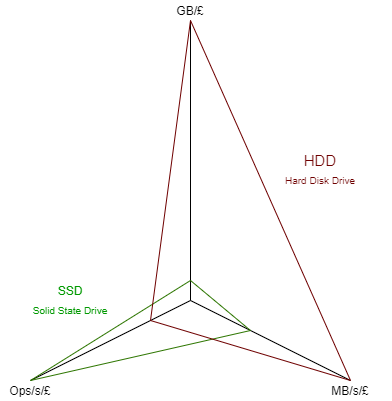
\includegraphics[width=\textwidth]{SSD vs HDD.png}}
        \end{minipage}
    
    \section*{RAID}
        Disk performance has not kept pace with CPU performance, creating a bottleneck.
        Redundant Array of Inexpensive Disks (\keyword{RAID}) increases disk based system 
        performance by using many disks in parallel.
        \compitem{
            \item An array fo physical drives appears as a single virtual drive.
            \item Distributes stored data over physical disks to allow parallel operation, improving performance.
            \item Use redundant disk capacity to respond to disk failure (more disks means lower mean-time-to-failure, more disks, higher chance a single disk in the group fails).
        }
        There are several levels of \keyword{RAID}, each with differing performance, redundancy and space-efficiency/cost.
        
        \subsection*{RAID 0 - Striping}
            \centerimage{width=\textwidth}{RAID 0.png}
            \compitem{
                \item Spread blocks in round robin fashion across disks.
                \item Can concurrently seek/transfer data (provided blocks on different physical disks).
                \item Can balance load across disks (sometimes).
                \item No redundancy (any disk failure will result in data being lost).
            }
        \subsection*{RAID 1 - Mirroring}
            \centerimage{width=\textwidth}{RAID 1.png}
            Mirror Data across disks to increase redundancy.
            \compitem{
                \item Reads can be serviced by either disk (e.g can read $0,1,2,3,4,5,6,7$ at the same time).
                \item Writes must update both disks in parallel (e.g can effectively only write to 4 disks at a time). (Slower)
                \item Failure recovery is easy (when a disk fails, use its mirror).
                \item Low space efficiency and hence high cost (store everything twice).
            }

        \subsection*{RAID 2 - Bit-Level Hamming}
            \sidenote{Hamming Codes}{
                A family of error correcting codes that make use of hamming distance (number of bits different between two patterns) to correct single bit errors.
                \centerimage{width=0.7\textwidth}{hamming.png}
                More complex codes can be used to check larger bit patterns with very few bits. The general algorithms can be seen \href{https://en.wikipedia.org/wiki/Hamming\_code\#General\_algorithm}{here}
            }
            \centerimage{width=0.9\textwidth}{RAID 2.png}
            Parallel access by striping at the bit level. 
            \compitem{
                \item Consecutive (in this case 4) bits are read in parallel, hence very high throughput (always reading/writing in parallel).
                \item Hamming error-correcting codes used to detect and correct single bit errors (can detect but not correct double bit errors).
                \item Cannot process requests in parallel (each request requires all disks, no concurrency).
                \item High storage overhead (less space efficient, increasing cost).
                \item Large number of writes as the error correcting codes must be updated (can become a bottleneck) \& every disk must write for every write operation.
            }
        
        \subsection*{RAID 3 - Byte-Level XOR}
            A single parity strip used (data on other disks XORed together).
            \centerimage{width=0.9\textwidth}{RAID 3.png}
            Can reconstruct missing data from parity and remaining data when a disk fails (disk reports).
            \compitem {
                \item Easy to reconstruct data when a disk fails
                \item More space efficient than \keyword{RAID 2}
                \item Only one I/O request at a time (but each request can be read in parallel from all disks)
            }

        \subsection*{RAID 4 - Block Level XOR}
            \centerimage{width=0.9\textwidth}{RAID 4.png}
            Parity Strip is XOR over blocks, allowing entire blocks to be accessed independently on different disks.
            \compitem {
                \item Allows read requests to be serviced concurrently.
                \item Low redundancy overhead.
                \item Parity must be updated after every single write, Parity disk becomes a bottlenecks
            }

        \subsection*{RAID 5 - Block Level Distributed XOR}
            \centerimage{width=\textwidth}{RAID 5.png}
            The most commonly used \keyword{RAID} level, by distributing parity there is potential for concurrency.
            \compitem {
                \item Some potential for write concurrency as parities are on different disks.
                \item Good storage/efficiency tradeoff.
                \item Reconstruction of disk is non-trivial (and slow).
            }

        \subsection*{RAID Level summary}
            Speeds compared with using a single disk.
            \begin{center}
                \begin{tabular}{c c c c c c c }
                    \multirow{2}{*}{\textbf{Category}} & \multirow{2}{*}{\textbf{Level}} & \multirow{2}{*}{\textbf{Description}} & \multicolumn{2}{c}{\textbf{I/O Data Transfer}} & \multicolumn{2}{c}{\textbf{I/O Request Rate}} \\
                    & & & Read & Write & Read & Write \\
                    \hline
                    Striping & 0 & Non-Redundant & \textcolor{green}{$\uparrow$} & \textcolor{green}{$\uparrow$} & \textcolor{green}{$\uparrow$} & \textcolor{green}{$\uparrow$} \\
                    Mirroring & 1 & Mirrored & \textcolor{green}{$\uparrow$} & \textcolor{orange}{$=$} & \textcolor{green}{$\uparrow$} & \textcolor{orange}{$=$} \\
                    \multirow{2}{*}{Parallel Access} & 2 & Redundant (Hamming ECC) & \textcolor{green}{$\uparrow$} \textcolor{green}{$\uparrow$} & \textcolor{green}{$\uparrow$} \textcolor{green}{$\uparrow$} & \textcolor{orange}{$=$} & \textcolor{orange}{$=$} \\
                    & 3 & Redundant (Bit Interleaved Parity) & \textcolor{green}{$\uparrow$} \textcolor{green}{$\uparrow$} & \textcolor{green}{$\uparrow$} \textcolor{green}{$\uparrow$} & \textcolor{orange}{$=$} & \textcolor{orange}{$=$} \\
                    \multirow{2}{*}{Independent Access} & 4 & Block interleaved Parity & \textcolor{green}{$\uparrow$} & \textcolor{red}{$\downarrow$} & \textcolor{green}{$\uparrow$} & \textcolor{red}{$\downarrow$} \\
                    & 5 & Block interleaved distributed parity & \textcolor{green}{$\uparrow$} & \textcolor{red}{$\downarrow$} & \textcolor{green}{$\uparrow$} & \textcolor{orange}{$=$} or \textcolor{red}{$\downarrow$} \\
                \end{tabular}
            \end{center}
    \section*{Disk Caching}
    \centerimage{width=0.3\textwidth}{block device cache.png}
        We can cache sectors of disk in main memory to reduce access times. 
        \compitem{
            \item Buffer contains copies of disk sectors.
            \item OS manages disk in terms of \keyword{blocks} which are likely much larger than sectors (so loads multiple sectors).
            \item Must ensure contents are saved in case of failure (e.g lazy writing is very complex).
            \item Cahce has finite space, so a replacement policy must be implemented.
        }
        \subsection*{(LRU) Least Recently Used}
            Replace the block that was in cache longest with no references. 
            \\
            \\ Cache is a stack of pointers to blocks in memory, when a block is 
            referenced, it is pushed to the top of the stack. Replacement evicts 
            the block at the bottom of the stack.
            \centerimage{width=0.8\textwidth}{lru block cache.png}
            This replacement policy does not track how many times a block is accessed, 
            only the relative time of the last access (through stack position).
        \subsection*{(LFU) Least Frequently Used}
            \compitem {
                \item Replace the block with the fewest references.
                \item Each block has a counter (incremented when referenced), the lowest counter block is evicted during replacement. 
                \item To avoid this, can use frequency based replacement.
            }
        
        \subsection*{Frequency-Based Replacement}
            \centerimage{width=0.8\textwidth}{freq based replacement.png}
            To prevent items that get a sudden burst of accesses from lingering 
            for a long time in the cache, we only increment the count when a 
            block is shuffled out of the \textbf{new} section.
    
    \section*{File Systems}
        File systems organise information. Their main objectives:
        \compitem {
            \bullpara{Non-volatile, long term storage}{}
            \bullpara{Sharing information}{e.g compilers, applications, text data etc.}
            \bullpara{Concurrent Access}{Many programs can access many files pesudo-simultaneously}
            \bullpara{Convenient Organisation}{symbolic names, directories}
            \bullpara{Easy management of data}{automatic backup, snapshots etc.}
            \bullpara{Security}{Permissions, read/write, hidden files}
        }

        \subsection*{File Naming}
            A \keyword{file} is an arbitrary size collection of data, extensions allow for easy identification of type from an identifier:
            \begin{center}
                \begin{tabular}{l l l}
                    \textbf{Type} & \textbf{Extension} & \textbf{Function} \\
                    \hline
                    executable & exe,com,bin,no extension & read \& load to run machine code program. \\
                    object & obj, o & compiled machine language, not linked. \\
                    source code & c, cpp, java, rs, py, s & Source code, extension identifies language. \\
                    batch/bash & bat (windows), sh (unix) & Script of commands to be interpreted by the terminal. \\
                    text & txt & Text data (usually \keyword{ascii}). \\
                    library & lib, a, so, dll & Libraries that programs can link to. \\
                    archive & arc, zip, tar & Compressed archives (for transmission or storage). \\
                \end{tabular}
            \end{center}

            There are also several types of file.
            \begin{center}
                \begin{tabular}{l p{14cm}}
                    \textbf{Type} & \textbf{Description} \\
                    \hline
                    Hard Links & A file that aliases the data of another file (refers 
                                 to the specific location of the data). \\
                    Soft Links & A soft/symbolic link aliases the path to a file 
                                 by another (e.g file points to another file, which 
                                 in turn points to its data). The \fun{ln} command can 
                                 be used to soft link files in unix based systems. \\
                    Regular & Normal file as discussed in the table above. \\
                    Directory  & A collection of files, that can itself be added to directories. \\
                    Character Special & A file that provides access to a character I/O device
                                        \\
                    Block Special  & Same as a character special file, but for block devices. \\
                \end{tabular}
            \end{center}

        \subsection*{Filesystem support functions}
            \compitem {
                \bullpara{Name Translation}{ Converting paths to disks \& blocks (logical) for use by the driver.}
                \bullpara{Management of Disk Space}{Allocating and deallocating storage for files.}
                \bullpara{File locking for exclusive access}{Important when many programs may access a fiule concurrently (can fuse the \fun{fcntl} syscall with the \const{F\_SETLK},\const{F\_SETLKW}, and \const{F\_GETLK})}
                \bullpara{Performance Optimisation}{Caching/Buffering}
                \bullpara{Protection against system failure}{Backup/Restore in case of a crash/power failure/unexpected shutdown}
                \bullpara{Security}{Enforcing file permissions}
            }
        
        \subsection*{File Attributes}
            \begin{itemize}
                \bullpara{Basic}{
                    \compitem{
                        \bullpara{File Name}{Symbolic name, unique in directory}
                        \bullpara{File Type}{e.g text, binary, executable, directory}
                        \bullpara{File Organisation}{placement of contents in blocks (sequential, random)}
                        \bullpara{File Creator}{program that created the file}
                    }
                }
                \bullpara{Address information}{
                    \compitem{
                        \bullpara{Volume}{Disk drive, partition}
                        \bullpara{Start Address}{cylinder, head, sector (logical block addressing information)}
                        \bullpara{Size Used}
                        \bullpara{Size Allocated}
                    }
                }
                \bullpara{Access Control Information}{ 
                    \compitem{
                        \bullpara{Owner}{User that controls the file}
                        \bullpara{Authentication}{Locked files may need a password/key}
                        \bullpara{permitted actions}{e.g read/write, dlete permissions (owner/others)}
                    }
                }
                \bullpara{Usage Information}{ Metadata for paper-trail.
                    \compitem{
                        \bullpara{Creation Timestamp}{Date \& Time}
                        \bullpara{Last Modified}{(can include the user that made the modification)}
                        \bullpara{Last Read}{}
                        \bullpara{Last Archived}{For keeping track of backups}
                        \bullpara{Expiry Date}{For automatic deletion (e.g recycle bin contents)}
                        \bullpara{Access activity}{Metadata for reads/writes etc. (can be used in improving performance)}
                    }
                }
            \end{itemize}

        \subsection*{Unix/Linux Files}
            \subsubsection*{Common Filesystem Syscalls}
                \codelist{C}{file syscalls.c}
            \subsubsection*{File Attributes}
                \centerimage{width=\textwidth}{file attr triads.png}
                \codelist{Bash}{result.sh}
        
    \section*{File System Organisation}
            \subsection*{Space Allocation}
                File size is variable (can increase or decrease) and is allocated on the disk in blocks (usually $512 \to 8192$ bytes). The block size is determined by the file system.
                \\
                \\ \begin{minipage}[t]{0.5\textwidth}
                    \centerline{\textbf{Block Size too Small}}
                    \compitem{
                        \item High overhead for managing large files (large number of blocks to keep track of)
                        \item High file transfer time (large file $\to$ lots of blocks across the disk $\to$ lots of seeking back and forth)
                    }
                \end{minipage}
                \begin{minipage}[t]{0.5\textwidth}
                    \centerline{\textbf{Block Size too Large}}
                    \compitem {
                        \item Internal fragmentation (Files leave parts of large blocks unused - wasteful)
                        \item Small files waste lots of space.
                        \item Caching is based on blocks, so end up having a very large cache space, or unable to cache many blocks.
                    }
                \end{minipage}
            \subsection*{Contiguous File Allocation}
                Place file data on a contiguous stretch of addresses on storage device. Similar to segment based memory management.
                \compitem {
                    \item Successive logical records are usually physically adjacent, reducing seek time when reading the file (seek to start, then just traverse file).
                    \item External Fragmentation can occur (unused blocks between files).
                    \item If unable to allocate new blocks as a file grows, must transfer to new large free section (expensive, requires lots of I/O).
                }
                \centerimage{width=\textwidth}{contiguous file allocation.png}
            \subsection*{Block Linkage/Chaining}
                Each file contains a linked list of blocks. When locating a block, traverse the linked list to by seeking to block, reading pointer.
                \compitem{
                    \item Can grow files without expensive re-allocation (just set pointer of end block to point to a newly allocated one).
                    \item No external fragmentation (as all blocks can be used in any order, by any file).
                    \item Space used for pointer in each block.
                    \item Traversing files requires lots of seeking from block to block.
                    \item For small block sizes the number of seeks to traverse a file increases.
                }
                \centerimage{width=\textwidth}{block linkage allocation.png}
            \subsection*{Block Allocation Table}
                Uses a directory mapping files to first block. Table maps blocks to the next block in the file, indicating free spots (\const{FREE}) and block with no next (end of file - \const{NULL}).
                \compitem{
                    \item File allocation table can be cached in memory for fast lookup.
                    \item Does not require lengthy seeks to traverse the block numbers for the file.
                    \item No external fragmentation.
                    \item However files can become fragmented (spread across disk) which reduces read/write speed (e.g must do lots of seeks to read the whole file), so should be periodically defragmented (disk reorganised to place files blocks next to eachother, very expensive operation).
                    \item Table can become impractically large, using up lots of memory, and more than one block of storage.
                }
                \centerimage{width=\textwidth}{block allocation table.png}
                This system is used for \keyword{microsoft}'s \keyword{FAT16/32} file system (with the table cached in memory).
            \subsection*{Index Blocks}
                Each table has one or more index blocks. Index blocks contain an array of pointers to data blocks, and pointers to subsequent index blocks.
                Basically page tables for file systems. The example below has miniscule index blocks for illustration purposes.
                \compitem {
                    \item Can search through index blocks to find location fo file blocks easily.
                    \item No external fragmentation \& can extend files easily.
                    \item Index blocks can be cached in memory just like data blocks.
                    \item Index blocks are per-file, hence can load file's table, rather than have an enormous global table as with \keyword{FAT}
                }
                \centerimage{width=0.9\textwidth}{index blocks.png}

            \subsection*{Linux Inodes}
                Linux/Unix uses the \keyword{Index Blocks} strategy through \keyword{inodes} (index nodes).
                \\
                \\ Inode contain:
                \compitem {
                    \item Type \& Access control.
                    \item Number of links to that inode.
                    \item User \& Group ID.
                    \item Access \& Modification time.
                    \item Inode change time (e.g when permissions, data stored in inode were changed).
                    \item Direct, Indirect, Double Indirect \& Triple Indirect pointers to data blocks.
                }

                The \struct{inode} struct can be found \href{https://github.com/torvalds/linux/blob/86085fe79e3c1a66e32f2acae0ae64f4cceb8d28/include/linux/fs.h#L620}{here} in the linux kernel.
                \codelist{C}{inode.h}
\end{document}
